% Copyright 2004 by Till Tantau <tantau@users.sourceforge.net>.
%
% In principle, this file can be redistributed and/or modified under
% the terms of the GNU Public License, version 2.
%
% However, this file is supposed to be a template to be modified
% for your own needs. For this reason, if you use this file as a
% template and not specifically distribute it as part of a another
% package/program, I grant the extra permission to freely copy and
% modify this file as you see fit and even to delete this copyright
% notice. 

\documentclass{beamer}

\usepackage{media9}
% Replace the \documentclass declaration above
% with the following two lines to typeset your 
% lecture notes as a handout:
%\documentclass{article}
%\usepackage{beamerarticle}


% There are many different themes available for Beamer. A comprehensive
% list with examples is given here:
% http://deic.uab.es/~iblanes/beamer_gallery/index_by_theme.html
% You can uncomment the themes below if you would like to use a different
% one:
%\usetheme{AnnArbor}
%\usetheme{Antibes}
%\usetheme{Bergen}
%\usetheme{Berkeley}
%\usetheme{Berlin}
%\usetheme{Boadilla}
%\usetheme{boxes}
%\usetheme{CambridgeUS}
%\usetheme{Copenhagen}
%\usetheme{Darmstadt}
%\usetheme{default}
%\usetheme{Frankfurt}
%\usetheme{Goettingen}
%\usetheme{Hannover}
%\usetheme{Ilmenau}
%\usetheme{JuanLesPins}
%\usetheme{Luebeck}
%\usetheme{Madrid}
%\usetheme{Malmoe}
%\usetheme{Marburg}
\usetheme{Montpellier}
%\usetheme{PaloAlto}
%\usetheme{Pittsburgh}
%\usetheme{Rochester}
%\usetheme{Singapore}
%\usetheme{Szeged}
%\usetheme{Warsaw}

\title{Modelling Handedness as a Function of Cooperation and Competition}

% A subtitle is optional and this may be deleted
\subtitle{Or: How I Learned to Bow Down to My Left-Handed Overlords}

\author{Meridith Bartley \and John Ensley}
% - Give the names in the same order as the appear in the paper.
% - Use the \inst{?} command only if the authors have different
%   affiliation.

    % MERIDITH: I'm not sure if I can take off the number 1 for institution but I tried one way and messed it up so I undid that and just commented out the second institution....Yup.

\institute[The Pennsylvania State University] % (optional, but mostly needed)
{
  %
  Department of Statistics\\
  The Pennsylvania State University
  % \and
  % \inst{2}%
  % Department of Theoretical Philosophy\\
  % University of Elsewhere}
  }
% - Use the \inst command only if there are several affiliations.
% - Keep it simple, no one is interested in your street address.

\date{STAT 590 Presentation, December 2, 2014}
% - Either use conference name or its abbreviation.
% - Not really informative to the audience, more for people (including
%   yourself) who are reading the slides online

\subject{Statistical Modelling}
% This is only inserted into the PDF information catalog. Can be left
% out. 

% If you have a file called "university-logo-filename.xxx", where xxx
% is a graphic format that can be processed by latex or pdflatex,
% resp., then you can add a logo as follows:

\pgfdeclareimage[height=0.5cm]{university-logo}{plainmarks/twotonemarks/twobluemark.png}
\logo{\pgfuseimage{university-logo}}

% Delete this, if you do not want the table of contents to pop up at
% % the beginning of each subsection:
% \AtBeginSubsection[]
% {
%   \begin{frame}<beamer>{Outline}
%     \tableofcontents[currentsection,currentsubsection]
%   \end{frame}
% }

% JOHN: I don't like those navigation symbols
\setbeamertemplate{navigation symbols}{}

% Let's get started
\begin{document}

\begin{frame}
  \titlepage
\end{frame}

\begin{frame}{Outline}
  \tableofcontents
  % You might wish to add the option [pausesections]
\end{frame}

% Section and subsections will appear in the presentation overview
% and table of contents.
\section{Introduction}

    \subsection{History of Handedness}

    \begin{frame}{History of Handedness}%{Optional Subtitle}
      \begin{itemize}
      \item {
        10\% of population is left-handed. 
      }
      \item {
        Why hasn't this percentage reached equilibrium in populations at either:
        \begin{itemize}
          \item 50\%-50\% between left and right-handedness
          \item 100\% either left or right handed 
          \item Some other handedness ratio 
        \end{itemize}
      }
      \item{
      This paper proposes that hand preference may be influenced by costs and benefits of cooperation and competition during human evolution.
      }
      \end{itemize}
    \end{frame}

    % \subsection{Second Subsection}

    % % You can reveal the parts of a slide one at a time
    % % with the \pause command:
    % \begin{frame}{Second Slide Title}
    %   \begin{itemize}
    %   \item {
    %     First item.
    %     \pause % The slide will pause after showing the first item
    %   }
    %   \item {   
    %     Second item.
    %   }
    %   % You can also specify when the content should appear
    %   % by using <n->:
    %   \item<3-> {
    %     Third item.
    %   }
    %   \item<4-> {
    %     Fourth item.
    %   }
    %   % or you can use the \uncover command to reveal general
    %   % content (not just \items):
    %   \item<5-> {
    %     Fifth item. \uncover<6->{Extra text in the fifth item.}
    %   }
    %   \end{itemize}
    % \end{frame}

\section{Building the Model}

    %\subsection{Another Subsection}

    \begin{frame}{Building the Model}
    \begin{itemize}
      \item We want to model $l$, the proportion of lefties, over time.
    \end{itemize}
    \[
      \frac{dl}{dt} = (1-l)P_{RL}(l) - lP_{LR}(l)
    \]
    \begin{itemize}
      \item Assume $P_{RL}$ and $P_{LR}$ are symmetric.
    \end{itemize}
    \begin{equation}
      \frac{dl}{dt} = (1-l)P_{RL}(l) - lP_{RL}(1-l)
    \end{equation}
    \begin{itemize}
      \item Break $P_{RL}(l)$ into increasing and decreasing components.
    \end{itemize}
    \begin{equation}
      P_{RL}(l) = cP_{RL}^{\textrm{coop}}(l) + (1-c)P_{RL}^{\textrm{comp}}(l)
    \end{equation}
    \end{frame}

    \begin{frame}{Video}

    \end{frame}

\section{Comparing Model to Baseball Data}


    \begin{frame}{Using Athletics Data}
      \begin{block}{Ideally}
        Want to compare predicted equilibria of eq (1) to animal population data where cooperation is present.
        \begin{itemize}
            \item Quantification of cooperation and available data very depending on task 
          \end{itemize}  
      \end{block}
      \begin{block}{Proxy Situation}
        Within atheletics, data on handedness and cooperation are readily available.
      \end{block}
      \begin{block}{Baseball Rank Equation}
        \begin{equation}
        l_r = \frac{1}{2}\frac{l_{bg}N\text{ erfc}(\hat{s}_r-\Delta\hat{s})}{r}
      \end{equation}
      \end{block}
      
    \end{frame}


    \begin{frame}{Visualizations}
      \begin{figure}
        \centering
        \begin{minipage}{.5\textwidth}
            \centering
            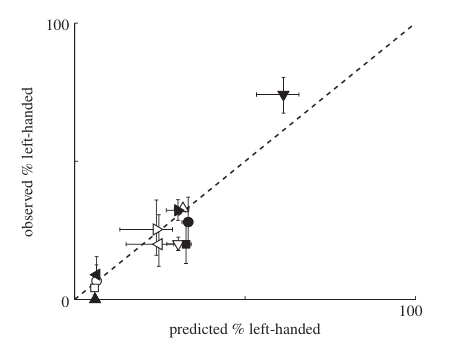
\includegraphics[width=1\linewidth]{ObVSPredLH}
            \caption{A subfigure}
        \end{minipage}%
        \begin{minipage}{.5\textwidth}
            \centering
            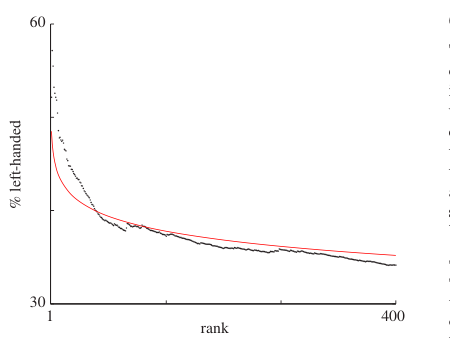
\includegraphics[width=1\linewidth]{CumuFracLH}
            \caption{A subfigure}
        \end{minipage}
        
    \end{figure}
    \end{frame}

% Placing a * after \section means it will not show in the
% outline or table of contents.
\section*{Summary}

\begin{frame}{Summary}
  \begin{itemize}
  \item
    Sports data may not be analogous to natural world data; \alert{further quantitative analysis with social animal groups} vital for future research.
  \item
    Analysis of athletics provides \alert{new insights into evolutionary origins} of handedness.
  \item
    This model may be \alert{applied to any species of animal} and may also be used in understanding \alert{other physical and/or behavioral lateralized adaptations}.
  \end{itemize}
  
  
\end{frame}



% All of the following is optional and typically not needed. 
\appendix
\section<presentation>*{\appendixname}
\subsection<presentation>*{For Further Reading}

\begin{frame}[allowframebreaks]
  \frametitle<presentation>{For Further Reading}
    
  \begin{thebibliography}{10}
  \beamertemplatearticlebibitems
  % Followed by interesting articles. Keep the list short. 

  \bibitem{Someone2000}
    Abrams, Daniel M. and Panaggio, Mark J.
    \newblock A model balancing cooperation and competition can explain our right-handed world and the dominance of left-handed athletes
    \newblock {\em Journal of The Royal Society Interface},
    2012.
  \end{thebibliography}
\end{frame}

\end{document}


